\documentclass[10pt,letterpaper]{article}

\usepackage{cogsci}
\usepackage{pslatex}
\usepackage[nodoi]{apacite}
\usepackage{graphicx}
\usepackage[american]{babel}
\usepackage{amsmath}
\usepackage[section]{placeins}
\usepackage{enumitem}
\usepackage{url}

\title{Understanding of linguistic politeness}
 
\author{{\large \bf Erica J. Yoon} \\
  \texttt{ejyoon@stanford.edu} \\
  Department of Psychology \\
  Stanford University}

\begin{document}

\maketitle

\begin{abstract}
To be added.

\textbf{Keywords:} 
Pragmatics; language; politeness; probabilistic model; cognition

\end{abstract}

\section{Introduction}

Communication is an act of cooperation between two or more partners \cite{grice1975logic}, and people normally assume that their communicators would speak in a way that is maximally truthful and informative. Imagine two people in a conversation, Tom and Sally, who are talking about pets they own. Tom says to Sally: ``I have two dogs.'' Assuming that Tom is a cooperative speaker, and that Sally also believes that he is, Sally will imagine the the true state of the world is such that Tom owns at least two dogs, which makes Tom's utterance truthful. Furthermore, she will infer that Tom owns two dogs, but not three or more, assuming Tom is informative and would have used a greater number term otherwise.

Now imagine the following situation: Tom and Sally are talking about a presentation that Sally just gave, and Sally asked for Tom's opinion on her talk. Tom says to Sally: ``It was okay.'' We can apply the same analysis as the previous one in this situation: if we assume Tom has some scale on his mind that ranges from `terrible' to `excellent,' and the term `okay' covers the positive part of the scale starting from the midpoint to the `excellent' end, then we might infer that Tom meant to indicate that Sally's presentation was ``above average but not excellent.''

But is that the farthest we can infer? For example, if Sally's performance was exactly average, would Tom necessarily use the word `average' instead of `okay' to be more informative and exact? Is it also possible that Tom used the word `okay' even though Sally's performance was actually below average? In that case, should we conclude that Tom was not a cooperative speaker? 

But people do share a strong intuition to maximize praise for their conversational partner, even by telling white lies and compromising truthfulness \cite{depaulo1998everyday}. Even children show tendency to tell white lies and think of white lies as better than malicious lies or even truths in situations in which the listener is harmed by truth-telling \cite{talwar2007white, bussey1999children}.

Past literature has explained this phenomenon of `linguistic politeness' in terms of people's want to maintain each other's `face': every human's wants to maintain positive public self-image and freedom from impositions. Going back to the example above, speakers maximize praises for the listener in order to save the listener's positive face, or self-esteem. Leech (1983) furthered this idea and proposed Politeness Principle (PP), which includes Maxim of Approbation: speakers must maximize praise and minimize dispraise for the listener. 

Despite the rich literature on related phenomena of linguistic politeness observed across different situations and cultures, there has thus far been few formal models for the common phenomenon of linguistic politeness. The goal of the current paper is to propose a generative model that looks at mechanisms of polite utterance generation and of listeners' inferences based on the utterances about speakers' underlying goals. 

\section{Model}
The current model\footnote{Link: \url{https://github.com/ejyoon/polite\_adj/blob/master/polite\_adj-model.txt}} is a variant of \citeA{kao2014nonliteral}'s model and follows its central assumptions: communicators are rational and cooperative agents, and listeners make inferences based on the assumption that speakers choose utterances to maximally achieve their communicative goals. The current model assumes there are two potential goals (and another goal that is combination of the two): the goal to convey the state, and goal to be polite. These goals are built in to the current model as possible QUD's.

The current model assume that there are ten possible states, which represent objective, evaluative scores for some item (e.g., Sally's presentation). The state of 0 denotes the worst possible score, 9 the best. This positive or negative association of states is formalized in the model in the form of valence prior, which is more likely for more desirable states (e.g., 9) and less likely for less desirable states (e.g., 0), Linguistic terms are assigned to particular state(s): ``bad'' denotes states of 0 and 1; ``not bad'' states of 2, 3, ..., 9; ``great'' states of 8 and 9, ``not great'' state of 0, 1, ..., 7. For the current, preliminary model, each word was mapped onto distinct states but not the others; this should be modified in the future to resemble more of a probabilistic distribution (see \citeNP{goodman2014probabilistic}).

Given this supposed scale of states and state-associated terms, let's imagine that there was only pressure to be truthful and informative for speakers. Then for the states 4 or 5, it would be equally likely for speakers to say either ``not bad'' or ``not great'' to describe the situation. However, with an additive pressure for speakers to be polite, ``not bad'' would be a better option than ``not great'' to describe the state of 4, assuming that, given the same amount of ambiguity, speakers would want to maximize praise (i.e., inclusion of maximally desirable state of 9 in ambiguity) and minimize dispraise (i.e., exclusion of minimally desirable state of 0). 

The current model hence sets up a prior for pressure to be polite, i.e., to obscure undesirability of states. Thus, the prior is high for lower, worse states because it is assumed that an undesirable state is more likely to induce the opposite wording from the speaker, e.g., a white lie. On the other hand, there is low pressure given higher, better states to obscure their truth value, since these states are desirable and therefore speakers would reason that listeners would be satisfied with accurate information about the true states.

Thus, the following is the question posed by `polite pressure prior' of the current model: given a state of X, how likely is it that the person would want to convey this or not? But one issue of this framing is that the pressure created by each state is not the \emph{cause} of a person being polite or impolite; it is rather the outcome of it. In the current experiments, the variable under question was how the perception of a speaker's politeness affects the way that listeners interpret different utterances. \emph{given} that a person is polite, then, the state determines how much the person would want to convey it truthfully. The future work should address how the model should address the discrepancy between pressure for politeness created by each state versus an individual speaker's politeness attribute.

The `literal listener' in the model hears an input utterance and draws QUD from QUD prior, and infers the state (0, 1, 2, ..., or 9) and politeness pressure level (which is for now binary: 0 for impolite and 1 for polite). The `speaker' reasons about this literal listener and outputs an utterance that aligns best with the given QUD. Then the `pragmatic listener' hears this speaker's utterance and infers the state and politeness level, taking into account speaker's reasoning about literal listener. Finally, `speaker2' accesses state and politeness as inferred by the pragmatic listener, and generates an utterance that most accurately conveys the speaker2's communicative goal to the pragmatic listener. 

The current work empirically tests the model's predictions for pragmatic listener (Figure \ref{fig:posteriormodel}), which are the following: ``bad,'' ``not bad,'' and ``not great'' produced by a polite speaker is more likely to indicate worse state than the same utterance produced by an impolite speaker; and ``great'' produced by an impolite speaker is more likely to indicate better state than the same produced by a polite speaker. 

\section{Evaluation}

\subsection{Prior distribution}

First, I collected data\footnote{Link: \url{https://langcog.stanford.edu/expts/EJY/polite\_adj/v1/polite\_adj\_statePrior.html}} to obtain judgments on prior distribution of likelihoods for listeners' judgments, i.e., judgments on listeners' ratings of presentations, poems, etc., when not given speakers' utterances. 25 subjects were recruited from Amazon's Mechanical Turk. Each subject read a scenario such as: ``Imagine that Kyle and James were talking about a presentation James just gave. James approached Kyle who saw James's presentation, and asked: ``How was my presentation?'' Before hearing Kyle's answer, how likely do you think James's presentation deserves each of the following scores?'' Subjects saw four scenarios with four different items in a random order: presentation, poem, cookie, and cake.  For each scenario, subjects rated the likelihood of each possible state from 0 to 9. The results are shown in Figure \ref{fig:prior}. This distribution was used for setting up the model priors for pre-utterance likelihood of each state. 

\begin{figure}
\begin{centering} 
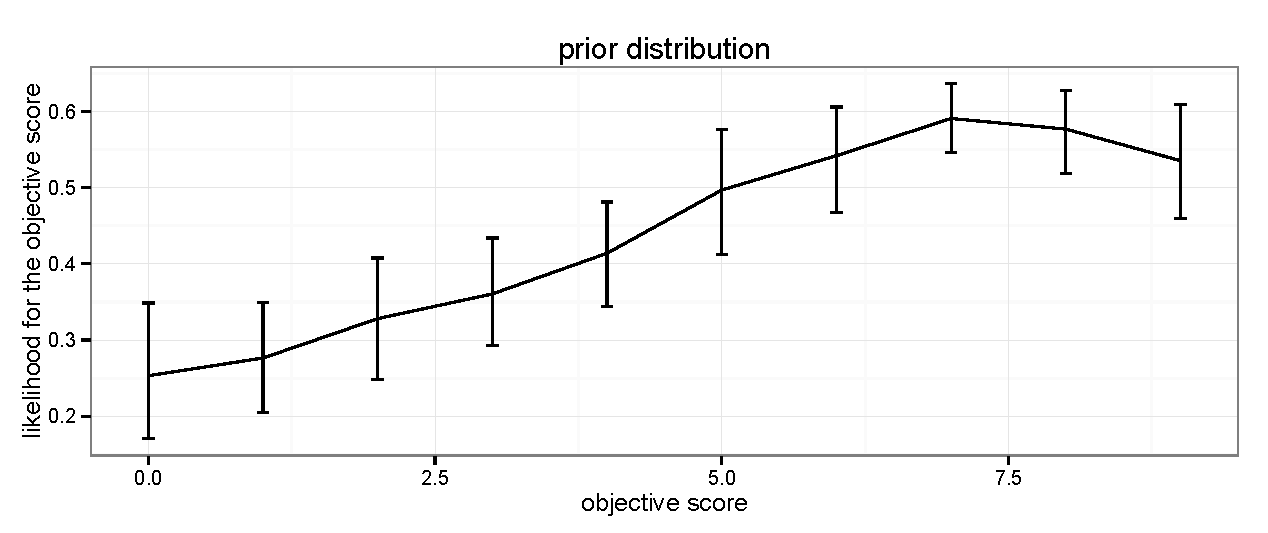
\includegraphics[width=3.2in]{figures/v1_statePrior.pdf}
\caption{\label{fig:prior} Prior likelihood distribution.}
\end{centering} 
\end{figure}

\subsection{Posterior distribution}

Next, I tested the predictions of the model for pragmatic listener's inferences about scores they deserve based on speakers' utterance and speakers' attributed politeness\footnote{Link: \url{https://langcog.stanford.edu/expts/EJY/polite\_adj/v2/polite\_adj\_statePos.html}}. 45 subjects were recruited from Amazon's Mechanical Turk, for three between-subjects conditions: (1) polite speaker condition; (2) impolite speaker condition; (3) baseline condition (in which no information about speaker's politeness was given). For example, in the polite speaker condition, subjects read a scenario such as: ``Imagine that Kyle and James were talking about a presentation James just gave. Kyle is a very polite person. James approached Kyle who saw James's presentation, and asked: ``How was my presentation?'' Before hearing Kyle's answer, how likely do you think James's presentation deserves each of the following scores?'' Subjects saw four scenarios with four different items (same as above) and four different utterances, ``great,'' ``not great,'' ``bad,'' and ``not bad,'' in a counterbalanced order. For each scenario, subjects rated the likelihood of each possible state from 0 to 9.

% analysis for exp 2 correlation between model and exit?

\begin{figure*}[t]
	\center{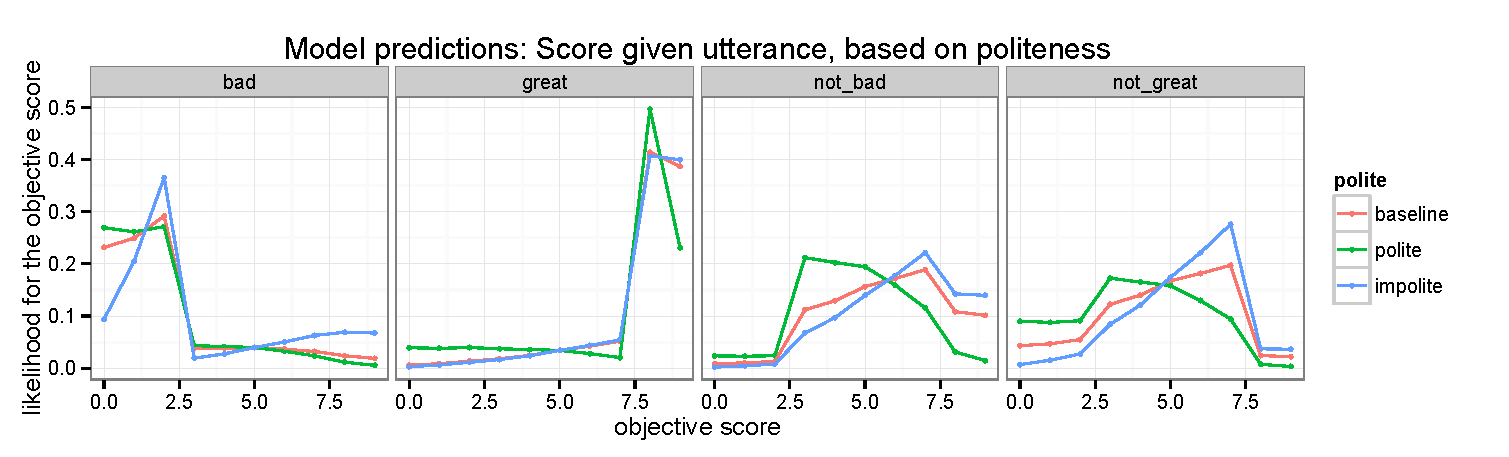
\includegraphics[width=.8\textwidth]{figures/v2_statePosterior_model.pdf}}
	\caption{\label{fig:posteriormodel} Model predictions for the posterior likelihood distribution.}
\end{figure*}

\begin{figure*}[t]
	\center{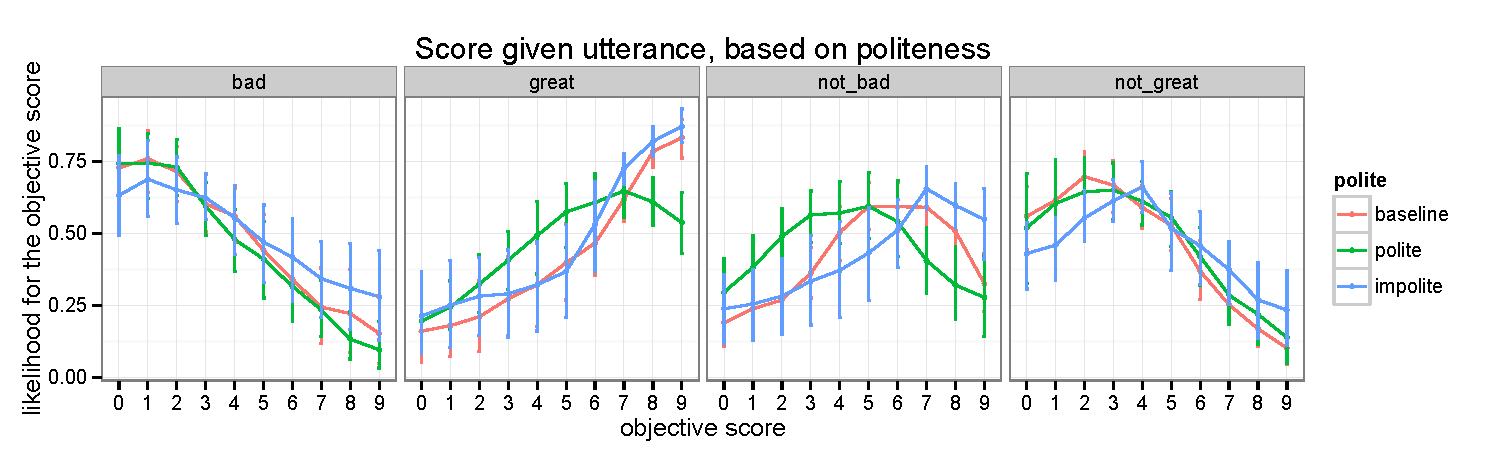
\includegraphics[width=.8\textwidth]{figures/v2_statePosterior.pdf}}
	\caption{\label{fig:posterior} Posterior likelihood distribution, faceted by utterances; different colors indicate whether the speaker was described as `polite' or `impolite,' or there was no indication (baseline).}
\end{figure*}

\subsection{Results and Discussion}

Empirical data confirmed the predictions of the model. That is, subjects judged that ``bad,'' ``not bad,'' and ``not great'' produced by a polite speaker was more likely to indicate worse state than the same utterance produced by an impolite speaker; and ``great'' produced by an impolite speaker was more likely to indicate better state than the same produced by a polite speaker. 

However, there are some aspects of the empirical data that the model failed to capture: first, some abrupt peaks in the model that are absent from the data are probably due to the one-to-discrete-n mapping of words to states, rather than smoother probabilistic distribution. Second, the model reveals less of the asymmetry between utterance conditions, especially between ``not bad'' and ``not great'' conditions. For example, different degrees of politeness do not predict posterior likelihood distribution as much in the ``not great'' condition as in the ``not bad'' condition. These elements might need to be modified in the polite pressure prior or another factor that modulates it. 

\section{General Discussion}

The current work used a computational model of linguistic politeness to predict listeners' inferential behaviors accurately, namely that listeners interpret utterances differently depending on the speaker's attributed degree of politeness. Listeners take into account that whereas impolite speakers tend to be more truthful, especially in conveying states that are suboptimal, polite speakers tend to obscure undesirable states. Future work should address the predictions for speaker in the model: given a particular state (e.g., 5), what utterance would a speaker choose to say? This line of work will help integrate previous work on, and re-define, the notion of politeness in a more systematic and predictive manner.

\bibliographystyle{apacite}

\setlength{\bibleftmargin}{.125in}
\setlength{\bibindent}{-\bibleftmargin}

\bibliography{YoonPoliteAdj}


\end{document}
